\graphicspath{{exp_design/fig/}}
{
\tikzset{external/figure name/.add={exp_design/}{}}

\chapter{Experimental design}
\label{chap:exp_design}

    \section{Hardware}

    Introduce honeybee

    \FloatBarrier\section{Methodology}
        
        \paragraph
        As discussed in Chapter~\ref{chap:system_id}, 
        generating data for the parameter estimation techniques involves two distinct flight stages.
        Firstly, the multirotor hovers with the suspended payload to gather data for payload mass estimation.
        A velocity step setpoint is then commanded to stimulate the swinging payload system for cable length estimation.
        Hence, the same methodology used for simulations will be used for practical flights.

        \paragraph
        For the data-driven techniques, the generation of practical training and testing data
        also follows the same general methodology as simulated flights:
        \begin{enumerate}
            \item Data logging starts when the multirotor is armed
            \item Takeoff and hover with the multirotor
            \item Command velocity step setpoints
            \item Land the multirotor
            \item Data logging stops when the multirotor is disarmed
            \item Download the data log from the multirotor
            \item Split the data into separate training and testing periods
            \item Build a model from the training data
            \item Perform model predictions over the testing data to calculate an error metric
        \end{enumerate}

        \paragraph
        Figure~\ref{fig:honeybee_with_payload} shows the Honeybee multirotor with a suspended payload during a practical flight.
        Numerous flights were performed with different 
        payload masses, 
        cable lengths, 
        wind conditions, 
        and dynamic payloads.
        The system identification methods were then performed for these different use cases.
        
        \paragraph
        The major differences between the simulated and practical flights involve the attachment of the payload and wind disturbances.
        In simulations, the payload cable is attached to the exact \gls{CoM} of the multirotor.
        However, for practical flights the cable is attached slightly below the \gls{CoM} of Honeybee due to mechanical constraints.
        Practical flights are also influenced by wind disturbances which were not considered in simulations.
        The measurement noise experienced by a practical multirotor may also differ from the noise models used in simulations.

        \begin{figure}[!htb]
            \centering
            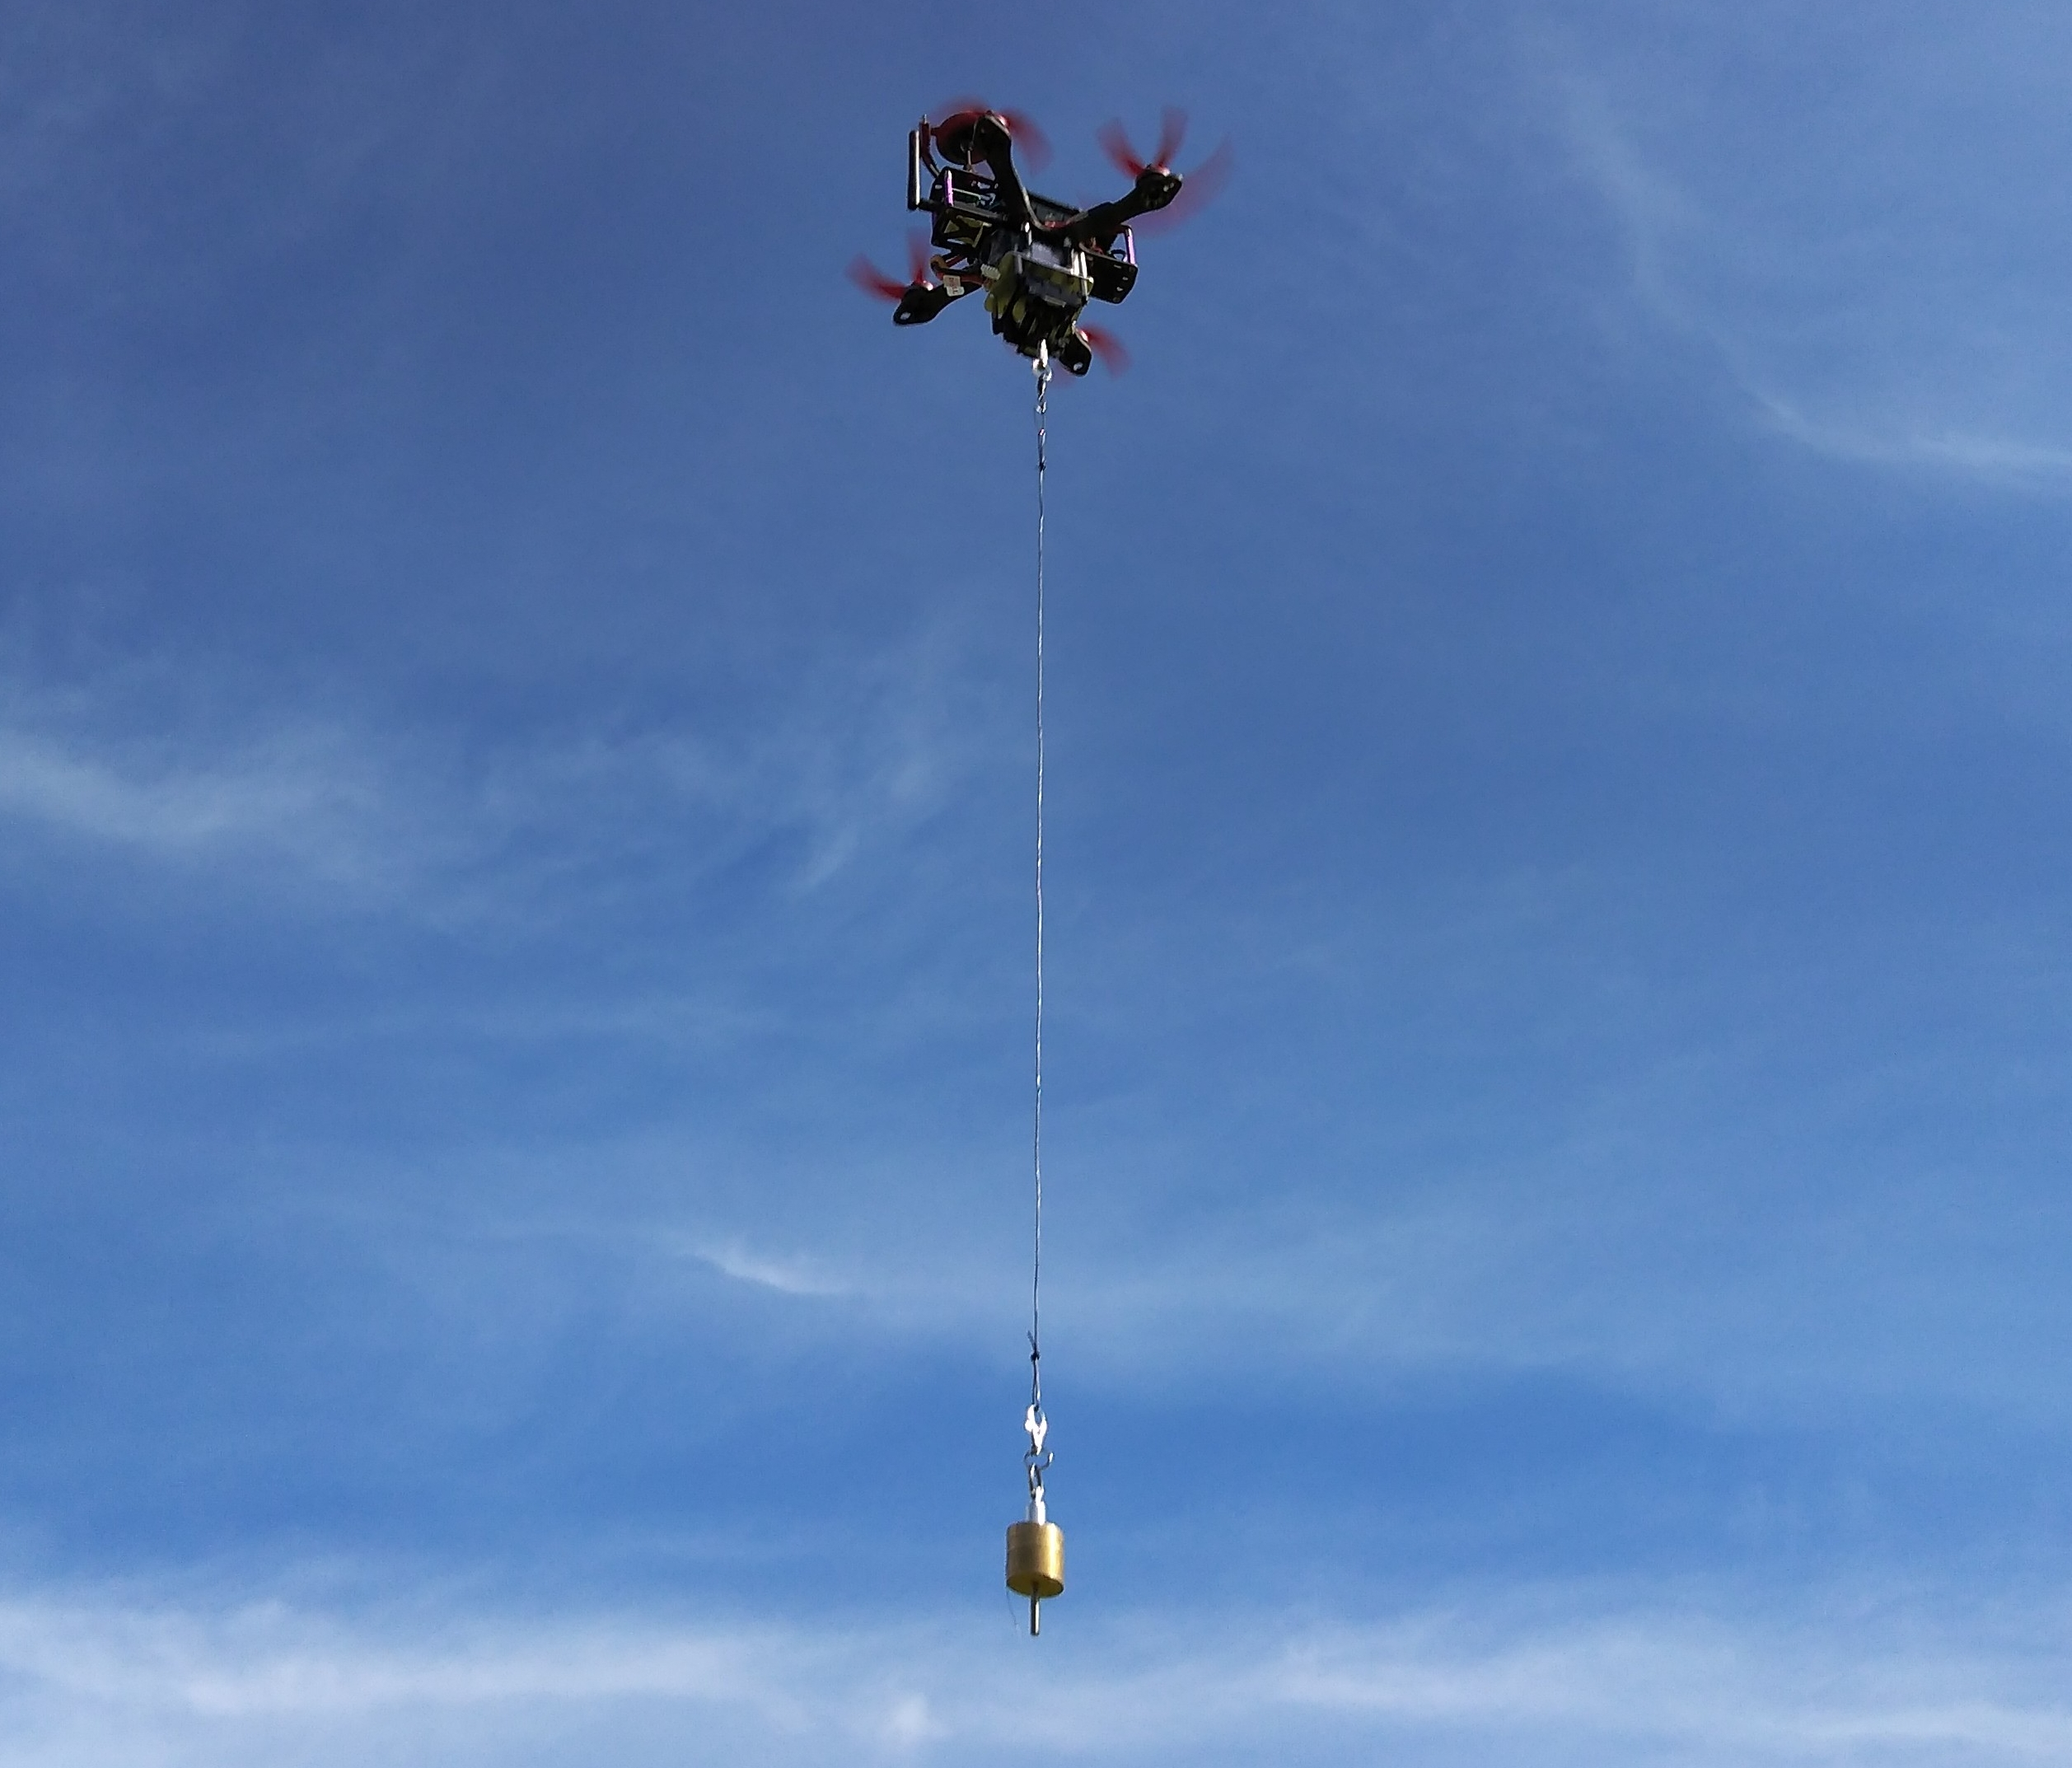
\includegraphics[width=0.5\linewidth]{honeybee_with_payload.jpg}
            \caption{Practical flight with Honeybee and a suspended payload}
            \label{fig:honeybee_with_payload}
        \end{figure}
    
    \section{Software}

    \section{HITL} \label{sec:exp_design_hitl}

    \paragraph
    MATLAB is used to generate a \gls{MPC} \gls{ROS} node 
    This \gls{ROS} node receives state feedback from the Gazebo simulator,
    computes the optimal control action,
    and sends the setpoint to PX4 through the package 'mavros'.

    \section{Practical flights}


}
